\documentclass[12pt]{article}
\usepackage{../lecture}
\lecture{5}{DFAs, NFAs, and Regular Expressions}
\date{February 9, 2021}

\begin{document}
\maketitle

\section{Equivalence of the DFAs, NFAs, and RegEx}
\begin{itemize}
    \item Theorem: Languages accepted by DFAs, NFAs, and regular expressions are the same.
    \begin{itemize}
        \item DFAs are special cases of NFAs.
        \item NFAs accept regular expressions.
        \item DFAs accept languages accepted by NFAs.
        \item Regular expressions for languages accepted by DFAs.
    \end{itemize}
\end{itemize}

\section{Thompson's Algorithm (RegEx to NFA)}
\begin{itemize}
    \item Concatenation is depicted by having the final state of the first expression $\epsilon$ transition to the starting state of the second expression.
    \item[] 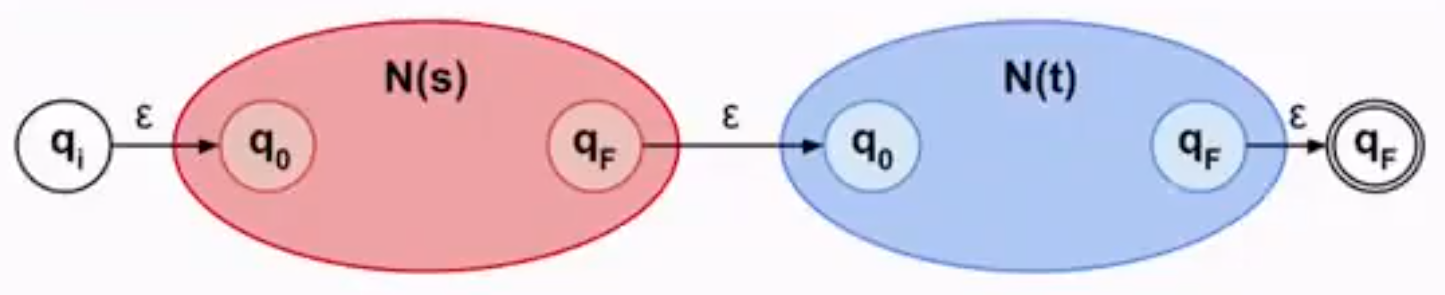
\includegraphics[width=0.9\linewidth]{images/thompson-concatenation.png}
    \item Union is depicted by having a new start state $\epsilon$ transition to both of the sub-start states and the both of the sub-final states $\epsilon$ transition to the new final state.
    \item[] 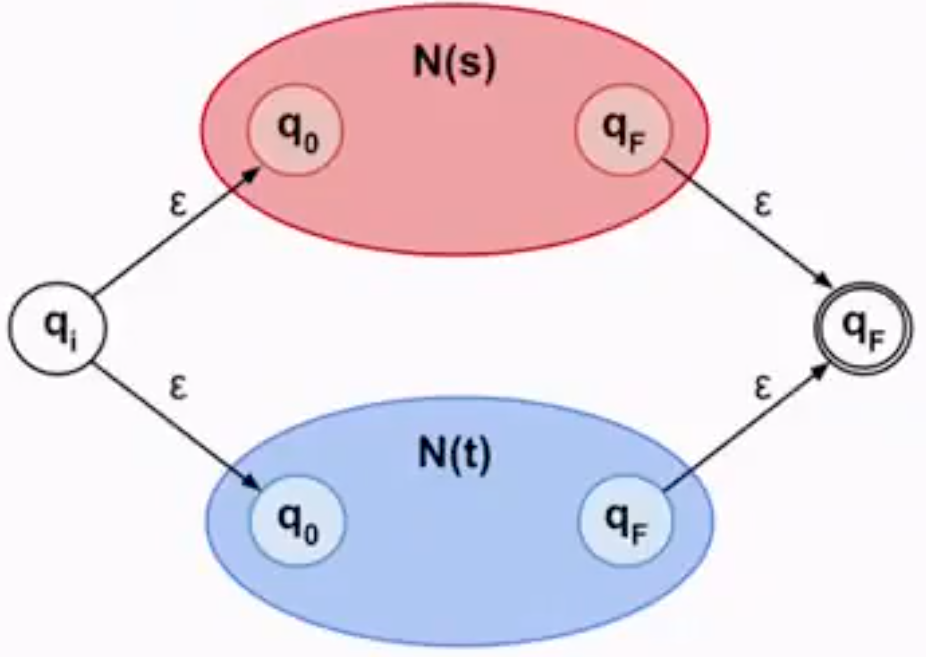
\includegraphics[width=0.6\linewidth]{images/thompson-union.png}
    \item Kleene start is depicted by having a new start state $\epsilon$ transition to the sub-start state and the new final state, as well as the sub-final state $\epsilon$ transition to the sub-start state and the new final state.
    \item[] 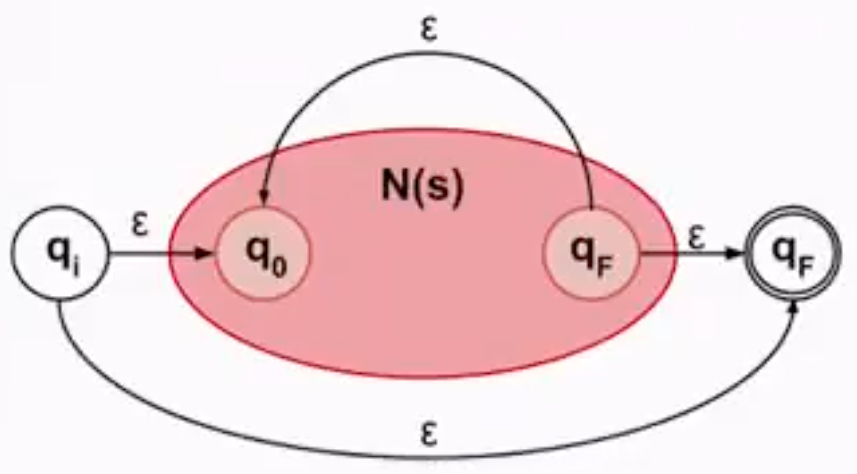
\includegraphics[width=0.6\linewidth]{images/thompson-kleene.png}
    \item Every regular expression has an equivalent NFA.
\end{itemize}

\section{Conversion of NFAs and DFAs}
\begin{itemize}
    \item Theorem: For every NFA $N$ there is a DFA $M$ such that $L(M) = L(N)$.
\end{itemize}

\subsection{DFAs are Memoryless}
\begin{itemize}
    \item DFA knows only its current state.
    \item The state is the memory.
    \item To design a DFA, answer the question: What minimal info is needed to solve the problem?
\end{itemize}

\subsection{The State of the NFA}
\begin{itemize}
    \item It is easy to state that the state of the automata is the states that it might be situated at.
    \item \textbf{configuration}: a set of states the automata might be in.
    \item Possible configurations: $\mathcal{P}(q) = \emptyset, \{ q_0, q_1 \}$.
    \item Big idea: Build a DFA on the configurations.
\end{itemize}

\subsection{Simulating an NFA by a DFA}
\begin{itemize}
    \item Think of a DFA with fixed memory that needs to simulate NFA $N$ on input $w$.
    \item For prefix $x$ of $w$, it needs to know at least $\delta^{\ast}(s, x)$, the set of states that $N$ could be in after reading $x$.
    \item The program should accept string $w$ if $\delta^{\ast}(s, w) \cap A \neq \emptyset$.
    \item Key Observation: DFA $M$ simulating $N$ should know current configuration of $N$.
    \item State space of the DFA is $\mathcal{P}(Q)$.
\end{itemize}

\subsection{Subset Construction}
\begin{itemize}
    \item NFA $N = (Q, \sum, s, \delta, A)$. We create a DFA $D = (Q', \sum, \delta', s', A')$ as follows:
    \begin{itemize}
        \item $Q' = \mathcal{P}(Q)$
        \item $s' = \epsilon reach(s)$
        \item $A' = \{ X \subseteq Q \mid X \cap A \neq \emptyset \}$
        \item $\delta'(X, a) = \bigcup_{q \in X} \delta^{\ast}(q, a)$
    \end{itemize}
\end{itemize}

\section{Converting an NFA into RegEx}
\begin{itemize}
    \item It is similar to the conversion from DFAs to regular expressions. The only difference is that NFAs contain $\epsilon$.
    \item Use the state removal method.
\end{itemize}

\end{document}
